%!TEX root = ../document.tex
\section{Implementation Ideas} \label{sec:IMPLEMENTATION_IDEAS}
%Lauritz
As described in Section~\ref{sec:PAPER_PROTOTYPE} and \ref{sec:FINAL_PROTOTYPE}, our proposed environment always presents relevant runtime data when developers interact with statements.
Just like in a debugger, when developers, for example, hover over identifiers in their application code, the IDE presents actual data, either objects or database rows.
However, in contrast to ordinary debugging environments, developers should not only be able to see the current state and step through the execution, but actually add and evaluate statements.
This should allow an interactive style of development centered around seeing the impact and effects of their code and queries immediately.
These features rely on the availability of runtime data.
First, developers can only see values and database entries for identifiers if such data is available.
Second, statements that might or might not embedd queries require referred variables and potentially even a database to run.
A realization of our idea would, therefore, implement components that gather the necessary data contexts from actual program runs as well as components that support developers in selecting interesting data contexts during development.

\subsection{Gathering Data Contexts}

Our approach depends on the availability of data contexts for the code sections of interest to the developer.
Such data contexts need to be realistic and immediately available to be useful.
Given these premises, two approaches could provide data contexts for specific code sections:
Either, deterministic test runs could establish data contexts on demand or tracing the application's execution could record data contexts in advance.
Running tests to provide the runtime during development would only require to store coverage information that associates code sections with test cases, while recording contextual information in advance implies storing as much data as necessary to actually run any statements in the sources of an application.
The time necessary for test execution depends on the granularity of the covering tests with a full spectrum from fine-grained, isolated unit tests to high-level, long-running acceptance tests.
Previously recorded data contexts, however, need just be fetched from a database, which could also be an in-memory database, and, thus, potentially provides faster access to data contexts compared to establishing runtime data through running tests.
Fetching recorded data context is further independent of the availability.
It could be captured in deployed systems used by real customers, which would also provide more realistic runtime data.

Assuming deterministic code, a reasonable tradeoff between space and time demands would be to record data not on the level of single statements but on the level of methods.
Such an implementation would record all data necessary to actually run a method with all its statements.
Such data includes provided parameters, accessible state, and the the database at the moment methods are entered, as shown in Figure~\ref{fig:context_recording}.

\begin{figure}
    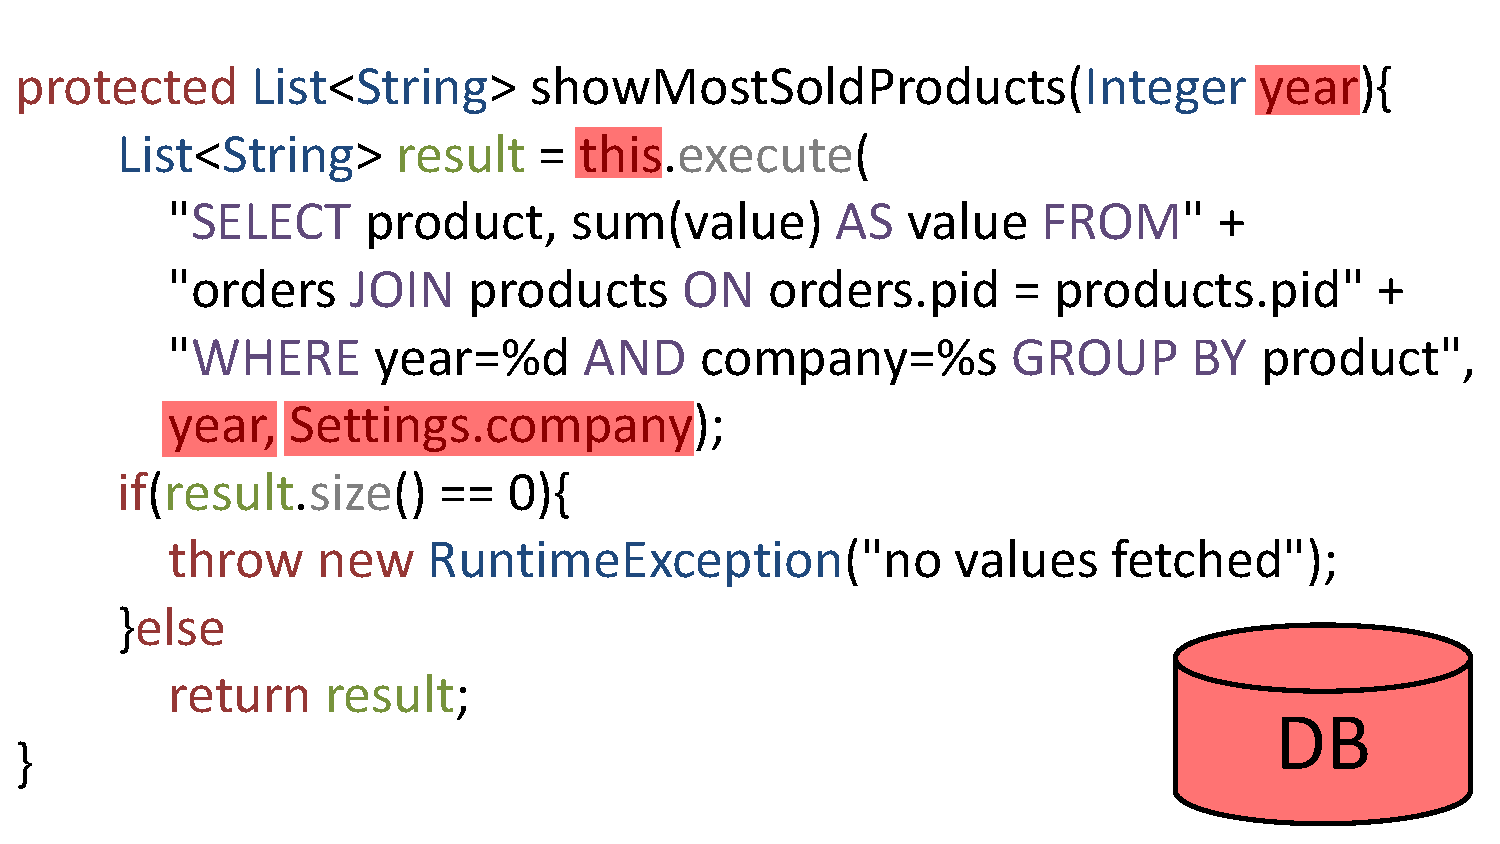
\includegraphics[width=\linewidth]{images/context}
    \caption{Running the statements of this Java method with its embedded SQL query requires the data highlighted in red: the parameter, accessible state, and the database.}
    \label{fig:context_recording}
\end{figure}

When a developer then interacts with a specific line in the method's body, we could use ordinary breakpoints to establish the necessary runtime data for that specific line of interest. 
Accessible state includes global state and, depending on the used programming language, also state from surrounding scopes as, for example, from surrounding functions.
Snapshots of the database are necessary as methods that embedd queries might modify the database, potentially impeding subsequent runs of that method during the interactive development.

We will assume the recording approach and method granularity for the remainder of our documentation.

\subsection{Selecting Data Contexts}

The presented tracing approach generates potentially numerous data contexts for each method.
Given our tool traces live systems deployed at customers, each user interaction might lead to recorded data contexts for all triggered executions.
Further, even when our tool only traces deterministic test runs once, particular methods might still be covered through multiple test cases or even be called multiple times in single test cases as, for example, the case with methods called from loops.
For these reasons, developers might be confronted with many data contexts for each statement of interest when using an implementation of our approach.
Further, as data contexts from the same trace probably overlap considerably, presenting all data contexts to the developer might reduce usability significantly.
Approaches addressing this issue include automatic selection of interesting samples after clustering all data contexts, preselection of interesting data contexts through expert users, and combinations of those two methods.
Clustering data contexts could be based on several dimensions, including:
\begin{itemize}
  \item size of the associated database snapshot
  \item control flow that lead to this context
  \item timestamp of this context
\end{itemize}
Nevertheless, even supporting developers with automatic clustering and stored preselections, our tool should also enable developers to explore the full extent of available contexts and to make the final decision on which specific data context they want to use during development.
